\section{Anisotropy and daily modulation}\label{sec:11.7}

At $45^\circ$N the dark-matter wind arrives from almost straight overhead when Cygnus crosses the meridian, and from close to the horizon twelve sidereal hours later (\cref{fig:1-daily}). A crystal fixed to the laboratory floor is therefore probed along different crystal directions in the course of each sidereal day. An isotropic target such as a liquid has the same rate in every orientation; a crystal responds differently along different crystal axes, so its rate follows the sidereal day. The size of the effect differs widely between crystals: below \SI{1}{\percent} in silicon, for electron recoils and for phonons alike, and \SI{6}{\percent} for multiphonon events in sapphire above a threshold of \SI{300}{meV}. Two factors set it, the angular structure of the crystal response and the sharpness with which the halo singles out one direction of $\vect{q}$, and the two can be computed separately, for the electronic responses of \cref{chap:10} and the nuclear responses of this chapter alike.

\subsection{Rate at fixed orientation}

Take a coupling through one density, the electron density of \cref{sec:10.1} or the nuclear operator of \cref{sec:11.1}, with a potential $\tilde V(q)$ that depends only on $|\vect{q}|$. The rate per unit target mass is \cref{eq:8.2-spectrum} with one row, $\mathfrak{D} = |\tilde V(q)|^2$, and the direction of $\vect{q}$ enters both the structure factor $S(\vect{q},\omega)$ and the velocity kernel $\int\dd^3v\,f_\chi(\vect{v})\,\delta(\omega - \omega_{\vect{q}})$. For elastic scattering, $\omega_{\vect{q}} = \vect{q}\cdot\vect{v} - q^2/2\mchi$ (\cref{eq:A.4-omegaq}), and the delta function becomes $q^{-1}\delta(\hat{\vect{q}}\cdot\vect{v} - \vmin)$ with $\vmin = \omega/q + q/2\mchi$ (\cref{eq:1.3-vmin}). The laboratory distribution is the galactic one shifted by the Earth's velocity, $f_\chi(\vect{v}) = f_{\mathrm{gal}}(\vect{v} + \vect{v}_{\mathrm{E}})$ (\cref{eq:1.2-flab}). Substituting $\vect{u} = \vect{v} + \vect{v}_{\mathrm{E}}$ turns the velocity integral into
\begin{equation*}
  \int\dd^3v\,f_\chi(\vect{v})\,\delta(\omega - \omega_{\vect{q}}) = \frac1q\int\dd^3u\,f_{\mathrm{gal}}(\vect{u})\,\delta\bigl(\hat{\vect{q}}\cdot\vect{u} - \vmin - v_{\mathrm{E}}\,\hat{\vect{q}}\cdot\hat{\vect{v}}_{\mathrm{E}}\bigr) = \frac1q\,\hat f_{\mathrm{gal}}\bigl(\vmin + v_{\mathrm{E}}x\bigr) ,
\end{equation*}
with $x = \hat{\vect{q}}\cdot\hat{\vect{v}}_{\mathrm{E}}$ the cosine of the angle between the momentum transfer and the Earth's velocity. The function $\hat f_{\mathrm{gal}}(s)$ is the integral of the isotropic galactic distribution over the plane $\hat{\vect{q}}\cdot\vect{u} = s$, the Radon transform of $f_{\mathrm{gal}}$. For the truncated Maxwellian of \cref{eq:1.2-fgal}, the two Gaussian integrals across the plane run over the disc $u_\perp^2 < v_{\mathrm{esc}}^2 - s^2$, and
\begin{equation*}
  \hat f_{\mathrm{gal}}(s) = \frac{\pi v_0^2}{N_{\mathrm{esc}}}\Bigl[\ee^{-s^2/v_0^2} - \ee^{-v_{\mathrm{esc}}^2/v_0^2}\Bigr]\,\Theta\bigl(v_{\mathrm{esc}} - |s|\bigr) ,
\end{equation*}
with $N_{\mathrm{esc}}$ of \cref{eq:1.2-nesc}. The halo enters only through this function of one variable, and the crystal only through $S(\vect{q},\omega)$ at fixed $|\vect{q}|$, a function on the sphere of directions.

Both factors are now expanded on the sphere. The halo factor is a function of $x$ alone and has a Legendre series, $\hat f_{\mathrm{gal}}(\vmin + v_{\mathrm{E}}x) = \sum_\ell\tfrac12(2\ell + 1)\,\mathcal{H}_\ell\,P_\ell(x)$, with coefficients
\begin{equation}
  \mathcal{H}_\ell(\vmin) = \int_{-1}^{1}\dd x\;P_\ell(x)\,\hat f_{\mathrm{gal}}\bigl(\vmin + v_{\mathrm{E}}x\bigr) ,
  \label{eq:11.7-ups}
\end{equation}
the multipoles of the halo. The crystal factor is expanded in real spherical harmonics $Y_{\ell m}$, the real and imaginary parts of those of \cref{app:C.3}, taken in crystal axes, with components $S_{\ell m}(|\vect{q}|,\omega) = \int\dd^2\hat{\vect{q}}\,Y_{\ell m}(\hat{\vect{q}})\,S(\vect{q},\omega)$. The addition theorem \cref{eq:C.3-addition} holds for the real harmonics too. It gives $\int\dd^2\hat{\vect{q}}\,P_\ell(\hat{\vect{q}}\cdot\hat{\vect{v}}_{\mathrm{E}})\,Y_{\ell'm}(\hat{\vect{q}}) = [4\pi/(2\ell + 1)]\,\delta_{\ell\ell'}\,Y_{\ell m}(\hat{\vect{v}}_{\mathrm{E}})$, and the angular integral pairs each multipole of the response with the halo multipole of the same order:
\begin{keyresult}[Rate of a crystal at fixed orientation]
\begin{equation}
  \frac{\dd\mathcal{R}}{\dd\omega}(t) = \frac{\rho_\chi}{\mchi\,\rho_T}\int\frac{q\,\dd q}{4\pi^2}\,|\tilde V(q)|^2\sum_{\ell m}\mathcal{H}_\ell\bigl(\vmin(q,\omega)\bigr)\,S_{\ell m}(q,\omega)\,Y_{\ell m}\bigl(\hat{\vect{v}}_{\mathrm{E}}(t)\bigr) ,
  \label{eq:11.7-rate}
\end{equation}
with $\hat{\vect{v}}_{\mathrm{E}}(t)$ the direction of the Earth's velocity in crystal axes, which turns with the sidereal day. For a cubic crystal the sum over $m$ at each order is one cubic harmonic $Y^{\mathrm{c}}_\ell$ of \cref{eq:C.3-cubic}, $\sum_mS_{\ell m}Y_{\ell m}(\hat{\vect{v}}_{\mathrm{E}}) = S_\ell\,Y^{\mathrm{c}}_\ell(\hat{\vect{v}}_{\mathrm{E}})$ with $S_\ell(|\vect{q}|,\omega) = \int\dd^2\hat{\vect{q}}\,Y^{\mathrm{c}}_\ell(\hat{\vect{q}})\,S(\vect{q},\omega)$, for $\ell \le 10$.
\end{keyresult}
\noindent The monopole term reproduces the isotropic rate. Since $\int_{-1}^1\dd x\,\hat f_{\mathrm{gal}}(\vmin + v_{\mathrm{E}}x)/2q$ is the average of the velocity integral over the directions of $\vect{q}$, which \cref{eq:A.8-eta} identified with $\eta/2q$, the zeroth halo multipole is the mean inverse speed, $\mathcal{H}_0(\vmin) = \eta(\vmin)$. With $S_{00}Y_{00} = \bar S$, the term $\ell = 0$ of \cref{eq:11.7-rate} is the isotropic rate of \cref{eq:A.8-eta}. The other terms carry all of the time dependence, through $Y_{\ell m}(\hat{\vect{v}}_{\mathrm{E}}(t))$, and each is weighted by the product of a property of the crystal, $S_{\ell m}$, and a property of the halo, $\mathcal{H}_\ell$. The same separation underlies the harmonic method of Al-Adulrazzaq and collaborators~\cite[Eqs.~(6), (10), (17)]{aladulrazzaq2026anisotropic}. Stratman and Lin integrate the same rate directly over the directions of $\vect{q}$~\cite[Eqs.~(28), (29), (31)]{stratman2025daily}. For a coupling with several rows, $|\tilde V|^2S$ becomes the contraction of \cref{eq:8.2-spectrum}; as long as $\mathfrak{D}_{ab}$ depends on $|\vect{q}|$ alone, each $S_{ab}$ is expanded in the same way. A coupling that depends on the dark-matter velocity puts powers of $\vect{v}$ under the velocity integral, and its halo factor is then no longer a function of $x$ alone.

How quickly the halo multipoles fall with $\ell$ decides how much of a crystal's anisotropy reaches the rate. With the standard halo of \cref{sec:1.2}, the ratio $\mathcal{H}_2/\mathcal{H}_0$ is 0.13, 0.37, 0.51 and 0.70 at $\vmin = 300$, 500, 600 and \SI{700}{km.s^{-1}}, while $\mathcal{H}_4/\mathcal{H}_0$ is only $-0.016$, $0.017$, $0.069$ and $0.27$. The reason is the shape of the halo factor. As a function of $x$ it is a Gaussian of width $v_0/v_{\mathrm{E}} = 0.95$, centered at $x = -\vmin/v_{\mathrm{E}}$: the momentum transfer prefers to point along the wind, against $\vect{v}_{\mathrm{E}}$, but only loosely, and a broad function has small high multipoles. Near the kinematic edge, $\vmin \to v_{\mathrm{esc}} + v_{\mathrm{E}}$, only a small cap of directions around $-\hat{\vect{v}}_{\mathrm{E}}$ is allowed, and every multipole approaches $\mathcal{H}_0$ in magnitude. At small $\vmin$ the preference reverses: a particle that needs only a small velocity component along $\vect{q}$ is best served by a $\vect{q}$ nearly perpendicular to its velocity, and $\mathcal{H}_2/\mathcal{H}_0 = -0.13$ at $\vmin = 0$. The quadrupole changes sign at $\vmin = \SI{196}{km.s^{-1}}$ and the hexadecapole at 138 and \SI{435}{km.s^{-1}}, so the phase of a modulation can flip with the mass or the energy deposited, as the annual modulation does at \SI{211}{km.s^{-1}} (\cref{sec:1.2}). The halo therefore filters the anisotropy of a crystal: the quadrupole passes at the level of tens of percent, the hexadecapole at a few percent, and the higher orders only for the fastest particles.

We measure the result by the daily-modulation amplitude
\begin{equation}
  A_{\mathrm{day}} = \frac{\mathcal{R}_{\mathrm{max}} - \mathcal{R}_{\mathrm{min}}}{\mathcal{R}_{\mathrm{max}} + \mathcal{R}_{\mathrm{min}}} ,
  \label{eq:11.7-Aday}
\end{equation}
the half-range of the rate over one sidereal day divided by its mean, for a rate integrated above a threshold. It depends on the crystal, on its mounting and on the latitude, which together fix the path of $\hat{\vect{v}}_{\mathrm{E}}(t)$ in crystal axes (\cref{eq:1.2-local}), and on the dark-matter mass and the threshold, which fix the values of $\vmin$ the rate samples.

\subsection{Selection rules}

The first restriction is evenness. With inversion symmetry, or with time-reversal symmetry, $S(\vect{q},\omega) = S(-\vect{q},\omega)$ (\cref{app:A.4}), and every component with odd $\ell$ vanishes. This holds in silicon, germanium and GaAs, with or without spin--orbit coupling, at every $|\vect{q}|$, every $\omega$ and every temperature, and for the loss function as well as for $S$. The odd halo multipoles are large, $\mathcal{H}_1/\mathcal{H}_0 = -0.54$ at \SI{300}{km.s^{-1}}, but no even response can use them.

A response with odd parts needs both symmetries broken, as in a magnetically ordered crystal without a center of inversion. For a density its odd part is then small at small momentum transfer. For $f \ne i$ the matrix element starts as $\langle f|n_e(\vect{q})|i\rangle = \ii\vect{q}\cdot\vect{d}_{fi} - \tfrac12q_\alpha q_\beta Q^{\alpha\beta}_{fi} + O(q^3)$, with $\vect{d}_{fi}$ and $Q^{\alpha\beta}_{fi}$ the matrix elements of $\sum_j\vect{r}_j$ and $\sum_jr^\alpha_jr^\beta_j$; the term of order zero vanishes by orthogonality. The difference between $\vect{q}$ and $-\vect{q}$ is the interference of the two leading terms,
\begin{equation*}
  |\langle f|n_e(\vect{q})|i\rangle|^2 - |\langle f|n_e(-\vect{q})|i\rangle|^2 = 2\,\Imag\bigl[(\vect{q}\cdot\vect{d}_{fi})\,q_\alpha q_\beta Q^{\alpha\beta*}_{fi}\bigr] + O(q^5) ,
\end{equation*}
which is of third order in $q$. Inversion forbids it, because $\vect{d}_{fi}$ connects states of opposite parity and $Q_{fi}$ states of the same parity; time reversal forbids it, because it makes both matrix elements real in a suitable basis. Where it survives, it multiplies the odd halo multipoles, and the rate acquires a part that is odd in the direction of the wind: opposite wind directions in crystal axes give it opposite signs. Such nonreciprocal targets are treated in \cref{sec:14.5}. A chiral crystal that keeps time reversal has an even $S$, and its two enantiomers modulate identically.

The second restriction is the point group. A function of direction invariant under the cubic group has no component with $\ell = 2$ (\cref{app:C.3}), so in silicon, germanium and GaAs the anisotropy of every response, electronic or nuclear, starts at $\ell = 4$ with $Y^{\mathrm{c}}_4$, followed by $Y^{\mathrm{c}}_6$ and $Y^{\mathrm{c}}_8$. A uniaxial crystal, such as trigonal sapphire or a hexagonal polytype of SiC, has one invariant direction, the $c$ axis $\hat{\vect{c}}$, and allows $\ell = 2$ with $m = 0$ about it. To this order the rate is $\mathcal{R}_0 + \mathcal{R}_2P_2(\hat{\vect{c}}\cdot\hat{\vect{v}}_{\mathrm{E}})$, the constant plus a constant times $\cos^2\theta_{\mathrm{lab}}$ that \cref{sec:1.2} wrote down by symmetry alone, and \cref{eq:11.7-rate} now supplies the two constants. At $\ell = 4$ a trigonal crystal adds terms with $|m| = 3$, and a hexagonal one first breaks the symmetry about $\hat{\vect{c}}$ at $\ell = 6$. Combined with the halo filter, the counting already explains the main pattern: for the same anisotropy of the response, a uniaxial crystal modulates through $\mathcal{H}_2$, a cubic one through $\mathcal{H}_4$, roughly ten times less except near the kinematic edge.

\subsection{Electronic anisotropy}

How anisotropic is the loss function of silicon? The covalent bonds point along the four $\langle111\rangle$ directions, the conduction-band minima lie along $\langle100\rangle$, and an electron--hole pair of a few eV made with a momentum transfer of a few keV feels both. \Cref{fig:11-aniso}(a) shows the ratio $L_4/L_0$ of the cubic-harmonic components of the loss function, in the empirical pseudopotential model of \cref{sec:3.3} that \cref{lim:10.1a} used, with the random-phase head of the dielectric matrix and no local fields. Each component is fitted to the loss function computed along ten directions of the irreducible wedge of the cube. The $k$ grid has the full cubic symmetry, so the components with $\ell = 2$ and odd $\ell$ vanish identically and cannot leak in as artifacts; refining it from $12^3$ to $16^3$ points changes $L_4/L_0$ by at most 0.01. At $q = q_0 = \SI{3.73}{keV}$ the ratio is 0.18 at \SI{3}{eV}, 0.05 at \SI{5}{eV} and below 0.01 above \SI{8}{eV}. The hexadecapole is not dominant: $L_6/L_0$ is of the same size, and near the gap the components beyond $\ell = 8$ carry an rms deviation of \SI{10}{\percent} of $\bar L$ or more, a sign of structure on small angular scales. Away from the gap the response is closer to that of a uniform gas, which has no preferred direction. GaAs, with the same lattice and a different basis, has components of the same size.

The halo multipoles now decide how much of this survives in the rate. \Cref{lim:11.7a} follows it at \SI{5}{eV} for a \SI{10}{MeV} particle. Wherever $\vmin$ is well below the kinematic edge, $\mathcal{H}_4/\mathcal{H}_0$ is a few percent and the anisotropic part of the rate at each $q$ stays below a few tenths of a percent, carried by the term $\ell = 4$ alone. Only near the edge, where the halo admits a narrow cone of directions, does the rate depend strongly on the direction of the wind, by tens of percent, and there the components $\ell \ge 6$ enter as well. Integrated over the spectrum of a \SI{2}{MeV} particle, the components combine into a daily modulation of about \SI{1}{\percent} (\cref{we:11-daily}).

These numbers are those of a model, and the model has two known gaps. The empirical pseudopotential reproduces the bands, not the wavefunctions at large momentum, and the calculation stops at $q = 2.8\,q_0$. Local fields add the crystal's own reciprocal vectors to the response at $q + \vect{G}$ and are known to change the direction-averaged rate by a factor of 1.3 to 1.5 at \SI{10}{MeV} (\cref{sec:10.2}); their effect on $L_4$ has not been computed. The cubic-harmonic components of the silicon loss function from a first-principles calculation with local fields, on a grid of directions fine enough for the structure near the gap, are therefore an open quantity. So, with them, is the electronic daily modulation of silicon beyond a model estimate. The calculation is specified in \cref{app:E.16}: the full-$\vect{q}$ loss function on Lebedev grids of increasing order, projected on $Y^{\mathrm{c}}_\ell$ for $\ell = 4$, 6 and 8, with the components $\ell = 1$, 2 and 3 as built-in tests that must vanish.

Evenness also settles a point in the literature. Al-Adulrazzaq and collaborators compute the electronic daily modulation of silicon and GaAs at \SI{10}{MeV} from the full loss function and find about one percent. They attribute the nearly sinusoidal shape of the signal at \SI{5}{eV}, with one period per sidereal day, to the dipole component of the loss function~\cite[Sect.~III\,B]{aladulrazzaq2026anisotropic}. The dipole component vanishes identically in both crystals, as do all odd components. A period of one sidereal day does not need $\ell = 1$: when the crystal axes are tilted with respect to the Earth's axis, $Y^{\mathrm{c}}_4(\hat{\vect{v}}_{\mathrm{E}}(t))$ contains every harmonic of the sidereal frequency up to the fourth, and which one dominates depends on the mounting. Their Migdal rate in the soft limit, in which the electronic and nuclear momenta separate, depends on the loss function only through its components with $\ell = 0$ and 2 at each $|\vect{k}|$~\cite[Eqs.~(37)--(41)]{aladulrazzaq2026anisotropic}. In a cubic crystal the component $\ell = 2$ vanishes at every $|\vect{k}|$, so the soft-limit Migdal rate of silicon, germanium and GaAs has no daily modulation at all. Their computed modulation of the Migdal rate is much smaller than that of the electron rate, as it must be, and any residue is numerical. Beyond the soft limit the Migdal response is the subject of \cref{chap:12}.

\subsection{Nuclear anisotropy}

The nuclear response carries its direction dependence in two places. In the incoherent approximation \cref{eq:11.3-inc}, each nucleus enters through its Debye--Waller exponent $2W_\kappa(\vect{q}) = \vect{q}\cdot B_\kappa\cdot\vect{q}$ (\cref{eq:5.6-W}) and through the spectrum $P^\kappa_1(\hat{\vect{q}},\omega)$, which is built from the density of states projected on $\hat{\vect{q}}$. Both are quadratic forms in $\hat{\vect{q}}$. The projected density of states is $\hat{\vect{q}}\cdot D_\kappa(\omega)\cdot\hat{\vect{q}}$, with the tensor
\begin{equation*}
  D^{\alpha\beta}_\kappa(\omega) = \frac1N\sum_{\vect{Q}\nu}\Real\bigl[e^\alpha_{\kappa\nu}(\vect{Q})\,e^{\beta}_{\kappa\nu}(\vect{Q})^*\bigr]\,\delta(\omega - \omega_{\vect{Q}\nu}) ,
\end{equation*}
whose trace is the atom-projected density of states $g_{\mathrm{ph},\kappa}(\omega)$ and whose integral against $\coth(\omega/2T)/(2M_\kappa\omega)$ is $B_\kappa$. Stratman and Lin write the incoherent response with this tensor and compute its daily modulation in sapphire and SiC~\cite[Eqs.~(18)--(24)]{stratman2025daily}. At a site of cubic symmetry every second-rank tensor is a multiple of the unit tensor (\cref{app:C.3}). Then $B_\kappa = \langle u_x^2\rangle\mathbb{1}$ and $D_\kappa = (g_{\mathrm{ph},\kappa}/3)\mathbb{1}$, and the direction of $\vect{q}$ drops out of \cref{eq:11.3-inc} term by term:
\begin{keyresult}[Isotropy of the incoherent response of cubic crystals]
If every nucleus sits at a site of cubic symmetry, the incoherent nuclear response \cref{eq:11.3-inc} is independent of the direction of $\vect{q}$ at every phonon order and every temperature. The direction dependence of the harmonic nuclear response of silicon, germanium, diamond and GaAs is entirely in its distinct part, the pair terms of \cref{eq:11.3-exact}.
\end{keyresult}
\noindent The temperature enters only through the Bose factors, which multiply each phonon by a scalar, so the statement holds at any $T$. The published tensors of Stratman and Lin show it to numerical precision: for silicon the three diagonal elements of $B_\kappa$ agree to $2\times10^{-4}$ and the off-diagonal ones are below \SI{e-7}{\angstrom^2}, and the two sites of GaAs agree to $8\times10^{-4}$. Their finding that the multiphonon rates of silicon and GaAs do not modulate~\cite[Sect.~IV]{stratman2025daily} is therefore exact within their approximation, not a numerical accident.

The anisotropy of the cubic nuclear response is entirely in the coherent terms, and \cref{sec:11.3} computed them. At long wavelength the one-phonon weight per direction is $\sum_\nu(\hat{\vect{q}}\cdot\hat{\vect{e}}_\nu)^2/c_\nu(\hat{\vect{q}})$ of \cref{eq:11.1-Sac}. With the measured elastic constants of \cref{sec:11.1} its component $\ell = 4$ is $S_4/S_0 = 0.028$, and $\ell = 6$ is below $10^{-3}$. The PBE force constants of \cref{sec:5.2} give $S_4/S_0 = 0.025$ for $q \le 0.3\,q_{\mathrm{BZ}}$, and the dispersion of the branches raises $|S_6/S_0|$ to 0.026 at $0.7\,q_{\mathrm{BZ}}$. Beyond the zone the one-phonon weight is strongly anisotropic. Near each reciprocal-lattice vector the acoustic phonons at $\vect{q} - \vect{G}$ are soft and their weight $1/\omega$ is large. The vectors $\vect{G}$ of a shell point in definite directions, and the weight is concentrated along them: just beyond the shell $|\vect{G}_{111}| = \SI{3.95}{keV} = 1.76\,q_{\mathrm{BZ}}$, at $q = 1.79\,q_{\mathrm{BZ}}$, $S_4/S_0 = -0.36$, and $S_6/S_0$ reaches $-0.49$ at $2.9\,q_{\mathrm{BZ}}$; beyond $5\,q_{\mathrm{BZ}}$, $|S_4/S_0|$ still reaches 0.2 and $|S_6/S_0|$ 0.4. The two-phonon weight, a sum over pairs of the square of a correlation, is less anisotropic, with $|S_4/S_0|$ and $|S_6/S_0|$ of about 0.1 at most. From three phonons on the incoherent part dominates, and the coherent corrections, and with them the anisotropy, are below \SI{3}{\percent} (\cref{sec:11.3}). These components come from the same force constants and the same pair correlations as the direction-averaged weights of \cref{sec:11.3}, and \cref{app:E.17} specifies their tabulation for silicon, germanium and GaAs, with the incoherent components $\ell \ge 4$ as a test that must vanish to numerical noise.

A cubic crystal therefore modulates through its nuclear response by less than \SI{1}{\percent}, and appreciably just at masses whose largest momentum transfer, $2\mchi v_{\mathrm{max}}$, ends close to a shell of reciprocal-lattice vectors, where the halo multipoles are large and one shell dominates. In silicon that happens near 1 and \SI{2}{MeV} (\cref{we:11-daily}). At other masses the shells inside the kinematic range contribute with alternating signs and largely cancel, and above a few MeV the incoherent part dominates the rate: the amplitude is \SI{0.04}{\percent} at 3 and \SI{4}{MeV} and $10^{-4}$ at 5 and \SI{10}{MeV}.

A crystal whose nuclei sit at sites of lower symmetry has an anisotropic incoherent response already. To first order in the anisotropy of $B_\kappa$, write $\vect{q}\cdot B_\kappa\cdot\vect{q} = q^2[\bar b_\kappa + \tfrac23\Delta b_\kappa P_2(\hat{\vect{c}}\cdot\hat{\vect{q}})]$ for a uniaxial site, with $\bar b_\kappa = \tfrac13\Tr B_\kappa$ and $\Delta b_\kappa = B^{cc}_\kappa - B^{aa}_\kappa$ the difference between the elements along and across the axis. The Poisson weight $p^{\mathrm{ph}}_n = \ee^{-2W_\kappa}(2W_\kappa)^n/n!$ of $n$ phonons (\cref{eq:5.6-poisson}) changes by $\delta(2W_\kappa)(n/2W_\kappa - 1)$ in its logarithm, so that
\begin{equation}
  \frac{\delta p^{\mathrm{ph}}_n}{p^{\mathrm{ph}}_n} = \bigl(n - 2\bar W_\kappa\bigr)\,\frac{2\Delta b_\kappa}{3\bar b_\kappa}\,P_2(\hat{\vect{c}}\cdot\hat{\vect{q}}) ,
  \label{eq:11.7-dw}
\end{equation}
with $2\bar W_\kappa = q^2\bar b_\kappa$. Orders below the mean phonon number lose weight along the axis of larger displacement and orders above it gain. A threshold well inside the multiphonon tail needs $n$ far above $2\bar W_\kappa$. The rate above it therefore inherits the anisotropy of $B_\kappa$ multiplied by the phonon number, while the projected spectrum $P^\kappa_1(\hat{\vect{q}},\omega)$ adds an anisotropy of its own whenever the threshold cuts through the phonon band. For sapphire the published tensors give, weighted with $A_\kappa^2$ over the four Al and six O sites of the cell, $B^{cc}/B^{aa} - 1 = +0.059$; for 2H-SiC only $+0.008$, because the larger displacement along the axis of the Si sites is partly offset by the C sites.

\begin{limitbox}[Daily modulation from the anisotropic response][lim:11.7a]
The rate of a crystal at fixed orientation pairs each multipole $S_{\ell m}$ of the response with the halo multipole $\mathcal{H}_\ell$ of the same order, $\dd\mathcal{R}/\dd\omega(t) = (\rho_\chi/\mchi\rho_T)\int q\,\dd q\,(4\pi^2)^{-1}|\tilde V|^2\sum_{\ell m}\mathcal{H}_\ell S_{\ell m}Y_{\ell m}(\hat{\vect{v}}_{\mathrm{E}}(t))$, \cref{eq:11.7-rate}, for the loss function~\cite[Eqs.~(10), (25)]{aladulrazzaq2026anisotropic} and for the incoherent nuclear response with direction-dependent Debye--Waller exponents and projected densities of states~\cite[Eqs.~(19), (24)]{stratman2025daily}. Its first anisotropic term is $\ell = 4$ in a cubic crystal and $\ell = 2$ in a uniaxial one.
\par\smallskip
{\centering
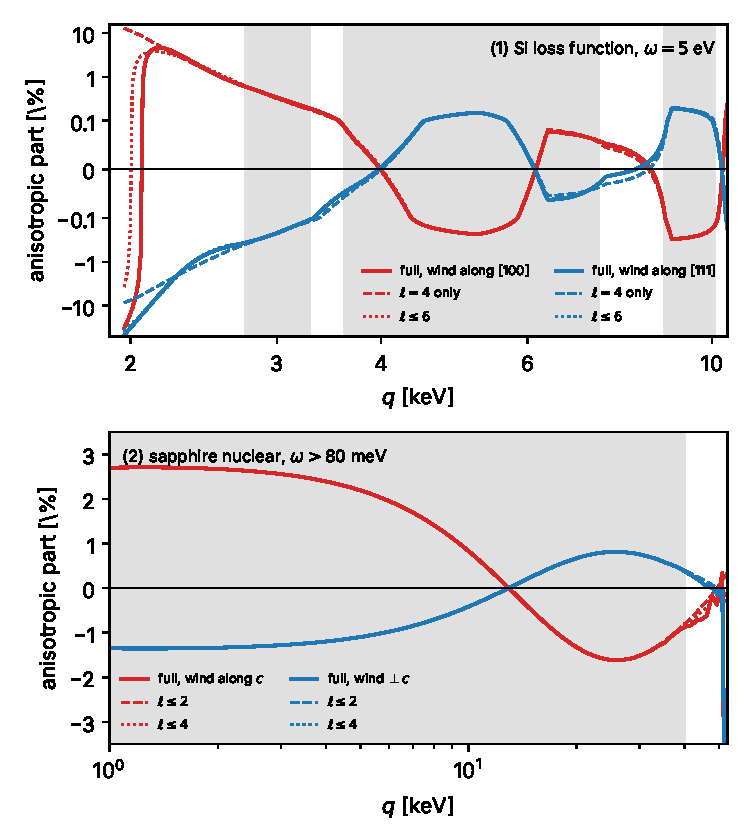
\includegraphics[width=\linewidth]{figures/ch11/limit11_7a.pdf}
\captionof{figure}{Anisotropic part of the rate at fixed momentum transfer for a wind along a fixed crystal axis, $\sum_{\ell \ge 1}\mathcal{H}_\ell\sum_mS_{\ell m}Y_{\ell m}(\hat{\vect{n}})/(\mathcal{H}_0S_{00}Y_{00})$ from \cref{eq:11.7-rate}, against $q$, for $\mchi = \SI{10}{MeV}$, a heavy mediator and the standard halo of \cref{sec:1.2}. (1) Silicon loss function at $\omega = \SI{5}{eV}$ in the empirical pseudopotential model (random-phase head, no local fields), wind along [100] (red) and [111] (blue), from the kinematic edge to the end of the model at $2.8\,q_0$; solid: all fitted components to $\ell = 8$; dashed: $\ell = 4$ alone, the formula; dotted: $\ell \le 6$, the leading correction (symmetric logarithmic axis, linear below \SI{0.1}{\percent}). (2) Sapphire, incoherent nuclear response with direction-dependent Debye--Waller exponents and projected densities of states from the site tensors of Stratman and Lin, integrated above \SI{80}{meV}, wind along the $c$ axis (red) and perpendicular to it (blue); solid: direct integral over the directions of $\vect{q}$; dashed: $\ell \le 2$, the formula; dotted: $\ell \le 4$. Gray bands: $q$ where the truncation at $\ell \le 4$ is within \SI{10}{\percent} of the full anisotropic part (or within $10^{-4}$ of the rate where that part is below $10^{-3}$): in panel (1) from \SI{2.7}{keV} up, except near 3.4, 8 and \SI{10}{keV}, where $\mathcal{H}_4$ or $L_4$ passes close to zero and $\ell = 6$ takes over; in panel (2) up to \SI{40}{keV}, against an edge at \SI{53}{keV}.}\label{fig:11-limit-7a}
\par}
\smallskip
Near the kinematic edge, where the halo admits only a narrow cone of directions, every multipole contributes, and a rate computed from the first anisotropic term alone misses the anisotropy there.
\end{limitbox}

\subsection{Daily-modulation amplitudes}

The time dependence comes from the path of $\hat{\vect{v}}_{\mathrm{E}}(t)$ in crystal axes. In equatorial axes the wind direction stays on a cone of half-angle $\theta_{\mathrm{E}} = 42.5^\circ$ around the Earth's rotation axis, and \cref{eq:1.2-local} gives its components along the local east, north and vertical. A crystal mounted with its axes along these three directions sees $\hat{\vect{v}}_{\mathrm{E}}(t)$ with exactly these components, and any other mounting is a fixed rotation of them. The amplitude of a term $\ell$ is then the range of $\sum_mS_{\ell m}Y_{\ell m}$ along the path. For a uniaxial crystal with its $c$ axis vertical at $45^\circ$N, the angle to the wind runs from $2.5^\circ$ to $87.5^\circ$, and $P_2$ sweeps from 0.997 to $-0.497$, nearly its full range. For a cubic crystal with [001] vertical at the same latitude, $Y^{\mathrm{c}}_4$ runs from $-0.39$ to $0.64$, close to its full range of $-0.43$ at [111] to $0.65$ at [100]. The rate oscillates mainly at twice the sidereal frequency, with a maximum when the wind arrives from overhead, along [001]. A cubic crystal mounted with [001] along the Earth's axis instead sees the wind circle at a fixed angle of $42.5^\circ$ from [001]. Then $Y^{\mathrm{c}}_4$ varies through its azimuthal part alone, $\cos4\varphi$, which gives four maxima per sidereal day and an amplitude six to ten times smaller.

\begin{figure}[tbp]
  \centering
  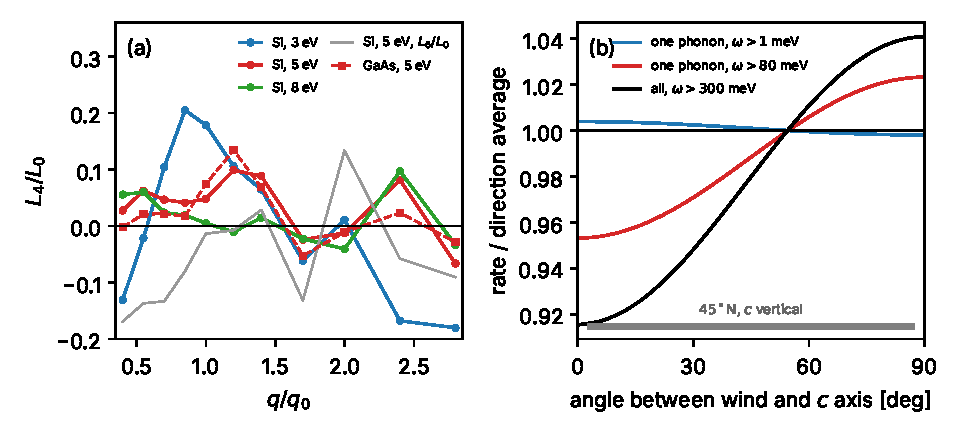
\includegraphics[width=\linewidth]{figures/ch11/fig11_7.pdf}
  \caption{Anisotropy of a cubic and of a uniaxial crystal. (a) Hexadecapole of the silicon loss function, the ratio $L_4/L_0$ of its components on the cubic harmonics $Y^{\mathrm{c}}_4$ and $Y^{\mathrm{c}}_0$, against $q/q_0$, $q_0 = \SI{3.73}{keV}$, at $\omega = 3$, 5 and \SI{8}{eV} (bins of \SI{1}{eV}); thin gray: $L_6/L_0$ at \SI{5}{eV}; dashed: GaAs at \SI{5}{eV}. Empirical pseudopotential model of \cref{sec:3.3}, head of the random-phase dielectric matrix, no local fields, ten directions of the irreducible wedge of the cube on a $k$ grid with the full cubic symmetry, components $\ell = 0$, 4, 6 and 8 fitted by least squares. (b) Rate of a sapphire crystal for a wind at a fixed angle to its $c$ axis, divided by the rate averaged over all wind directions, at $\mchi = \SI{10}{MeV}$ with a heavy mediator coupled to nucleon number: one phonon above \SI{1}{meV} (blue) and above \SI{80}{meV} (red), and all phonon numbers above \SI{300}{meV} (black). Incoherent nuclear response at $T = 0$ with the direction-dependent Debye--Waller exponents and projected densities of states of the published site tensors of Stratman and Lin~\cite{stratman2025daily}, whose $A_\kappa^2$-weighted anisotropy is $B^{cc}/B^{aa} - 1 = +0.059$. Bar: the range of angles swept in one sidereal day by a $c$ axis along the vertical at $45^\circ$N.}
  \label{fig:11-aniso}
\end{figure}

\Cref{fig:11-aniso}(b) shows the uniaxial case. Sapphire's rate depends on the direction of the wind almost only through the term $\ell = 2$, since the terms with $\ell \ge 4$ contribute less than $5\times10^{-4}$ of the rate, and its amplitude depends on which phonons the threshold admits. Above \SI{1}{meV}, where the acoustic and low optical phonons carry most of the one-phonon weight, the one-phonon rate along the axis and across it differ by \SI{0.6}{\percent}, and the rate of all phonon numbers by \SI{1.0}{\percent}, since these modes move all ten atoms of the cell almost isotropically. Above \SI{80}{meV} the highest optical modes alone remain, and they are polarized mostly in the basal plane: the one-phonon rate along the axis is \SI{7}{\percent} below the rate across it. Above \SI{300}{meV} the rate comes from three or more phonons, and \cref{eq:11.7-dw} multiplies the \SI{6}{\percent} anisotropy of the displacements by the phonon number: the difference grows to \SI{12}{\percent}. Mounted with its axis vertical at $45^\circ$N, a sapphire crystal then modulates with $A_{\mathrm{day}} = \SI{0.48}{\percent}$ for all phonons above \SI{1}{meV}, \SI{3.5}{\percent} for one phonon above \SI{80}{meV} and \SI{6.4}{\percent} above \SI{300}{meV}, at \SI{10}{MeV}. At \SI{30}{MeV} the amplitudes for the two higher thresholds fall to 1.2 and \SI{0.6}{\percent}. 2H-SiC, whose displacements are nearly isotropic, modulates less: 0.08, 0.61 and \SI{3.5}{\percent} for the same three cases at \SI{10}{MeV}. These are estimates within the incoherent approximation, which holds for $q$ above a few $q_{\mathrm{BZ}}$, here \SI{1.75}{keV} for the ten-atom cell of sapphire, and therefore for masses of a few MeV and above. They agree in pattern with the multiphonon calculation of Stratman and Lin, who find up to \SI{11}{\percent} in sapphire at \SI{10}{MeV} above \SI{300}{meV}, somewhat less in SiC and none in silicon and GaAs~\cite[Sect.~IV and App.~C]{stratman2025daily}. They use a different halo ($v_0 = 220$, $v_{\mathrm{esc}} = 500$ and $v_{\mathrm{E}} = \SI{240}{km.s^{-1}}$) and put the crystal axis along the wind at the start of the day. At lower masses the momentum transfers stay inside the zone, and the coherent single-phonon response decides the rate. The full phonon calculation of Griffin and collaborators finds daily modulation in sapphire of up to \SI{30}{\percent} at masses near \SI{50}{keV}, for a threshold that leaves only the optical branches. With the acoustic branches open it finds much less, because the sound speeds of sapphire are nearly isotropic~\cite[Sects.~III\,C and IV\,C]{griffin2018directional}. The same holds for the hexagonal polytypes of SiC, with the largest modulation in 2H~\cite[Sects.~IV\,B and V]{griffin2021sic}.

In silicon both the electron and the nucleon rates modulate, and with the same phase.

\begin{workedexample}{Daily modulation of a silicon crystal at $45^\circ$N}\label{we:11-daily}
A silicon crystal sits at latitude $45^\circ$N with [001] along the local vertical, [100] pointing east and [010] north. Dark matter of mass \SI{2}{MeV} scatters through a heavy mediator, either on electrons, through the loss function, or on nucleons, through the nuclear response. At this mass the momentum transfers reach $2\mchi v_{\mathrm{max}} = \SI{10.6}{keV} = 2.84\,q_0$; the electronic model ends at $2.8\,q_0$, and the sliver above it, at the kinematic edge where the rate vanishes, is dropped. The energy deposited on electrons stays below $\mchi v_{\mathrm{max}}^2/2 = \SI{7.0}{eV}$.

\emph{Geometry.} By \cref{eq:1.2-local}, the wind direction in crystal axes is
\begin{multline*}
  \hat{\vect{v}}_{\mathrm{E}} = \bigl(-\cos\delta_{\mathrm{E}}\sin h_{\mathrm{E}},\ \cos\ell_{\mathrm{lat}}\sin\delta_{\mathrm{E}} - \sin\ell_{\mathrm{lat}}\cos\delta_{\mathrm{E}}\cos h_{\mathrm{E}},\\
  \sin\ell_{\mathrm{lat}}\sin\delta_{\mathrm{E}} + \cos\ell_{\mathrm{lat}}\cos\delta_{\mathrm{E}}\cos h_{\mathrm{E}}\bigr) ,
\end{multline*}
with $\delta_{\mathrm{E}} = 47.5^\circ$ and the hour angle $h_{\mathrm{E}}$ advancing at the sidereal rate. Along this path $Y^{\mathrm{c}}_4$ of \cref{eq:C.3-cubic} runs from $-0.394$ to $0.640$, its maximum at $h_{\mathrm{E}} = 0$, when the wind arrives nearly along [001]. Let $\mathcal{R}_\ell$ be the term $\ell$ of \cref{eq:11.7-rate}, integrated over $q$ and $\omega$ without its factor $Y^{\mathrm{c}}_\ell$, and $\bar{\mathcal{R}}$ the rate averaged over orientations. If the hexadecapole dominates, $\mathcal{R}(t)/\bar{\mathcal{R}} = 1 + \sqrt{4\pi}\,(\mathcal{R}_4/\mathcal{R}_0)\,Y^{\mathrm{c}}_4(\hat{\vect{v}}_{\mathrm{E}}(t))$, and
\begin{equation*}
  A_{\mathrm{day}} = \sqrt{4\pi}\,\frac{0.640 + 0.394}{2}\,\frac{\mathcal{R}_4}{\mathcal{R}_0} = 1.83\,\frac{\mathcal{R}_4}{\mathcal{R}_0} .
\end{equation*}

\emph{Electronic part.} The integrals $\mathcal{R}_\ell = \sum_\omega\int\dd q\,q^3\mathcal{H}_\ell(\vmin)L_\ell(q,\omega)$ over the spectrum, with the components of \cref{fig:11-aniso}(a) in bins of \SI{1}{eV} from 1.5 to \SI{7.5}{eV}, give $\mathcal{R}_4/\mathcal{R}_0 = 4.9\times10^{-3}$, while $\mathcal{R}_6/\mathcal{R}_0 = -3\times10^{-5}$ and $\mathcal{R}_8/\mathcal{R}_0 = -7\times10^{-6}$ are negligible. The components beyond $\ell = 8$, which the ten directions do not resolve, enter with $\mathcal{H}_{10}$; estimated from the residual of the fit, they can shift the rate by about $10^{-3}$. The hexadecapole of the response, a few percent, passes because \SI{47}{\percent} of the rate of so light a particle comes from $\vmin > \SI{600}{km.s^{-1}}$, where the halo is sharp: weighted with the rate, $\mathcal{H}_4/\mathcal{H}_0$ is 0.09. The amplitude is $A_{\mathrm{day}} = 1.83\times4.9\times10^{-3} = \SI{0.9}{\percent}$, uncertain by about 0.1 percentage point from those higher components. The rate oscillates twice per sidereal day, with its maximum when Cygnus crosses the meridian.

\emph{Lattice part.} For the nucleon coupling, $\mathcal{R}_\ell = \sum_n\int\dd q\,q\,\mathcal{H}_\ell(q/2\mchi)\,\ee^{-2W}(2W)^n/n!\,s_{n,\ell}(q)$, with $2W = q^2\langle u_x^2\rangle$, $\langle u_x^2\rangle = \SI{2.45e-3}{\angstrom^2}$, and $s_{n,\ell}$ the cubic components of the exact one- and two-phonon weights of \cref{sec:11.3}, divided by their incoherent values; three and more phonons are treated as isotropic, their coherent corrections being below \SI{3}{\percent}. In $\vmin$ the deposit of $n$ phonons enters as $n\times\SI{30.4}{meV}/q$, the mean energy of the single-phonon distribution, which matters only at the smallest $q$, where the rate is small. The momentum transfers cross the shells $\vect{G}_{111}$ and $\vect{G}_{220}$, where the one-phonon weight is most anisotropic, and $\mathcal{R}_4/\mathcal{R}_0 = 3.2\times10^{-3}$, so $A_{\mathrm{day}} = \SI{0.58}{\percent}$, in phase with the electronic part since both $\mathcal{R}_4$ are positive. A detector that records both channels therefore sees an amplitude between 0.6 and \SI{0.9}{\percent}, the mean of the two weighted by their rates.

\emph{Mounting.} Over 3000 random orientations of the crystal at this latitude the largest amplitudes are 0.93 and \SI{0.60}{\percent}, so the vertical [001] is close to the best choice. With [001] along the Earth's axis instead, the wind circles at a fixed angle to [001], only the term $\cos4\varphi$ of $Y^{\mathrm{c}}_4$ varies, and the amplitudes drop to 0.15 and \SI{0.06}{\percent}, with four maxima per sidereal day.

\emph{GaAs.} The same mounting and mass give $\mathcal{R}_4/\mathcal{R}_0 = 3.8\times10^{-3}$ and $A_{\mathrm{day}} = \SI{0.7}{\percent}$ for the electronic part, in the same model and with the same uncertainty. For the nuclear part, with the one-phonon weights of the force constants of \cref{sec:5.5} and $\langle u_x^2\rangle \approx \SI{1.9e-3}{\angstrom^2}$, they give $\mathcal{R}_4/\mathcal{R}_0 = 1.6\times10^{-3}$ and $A_{\mathrm{day}} = \SI{0.29}{\percent}$. Both parts are in phase with those of silicon, and the combined amplitude of a GaAs detector lies between 0.3 and \SI{0.7}{\percent}.
\end{workedexample}

At \SI{1}{MeV}, where $2\mchi v_{\mathrm{max}} = \SI{5.3}{keV}$ lies just beyond the shell $\vect{G}_{111}$, the lattice amplitude of silicon is \SI{0.77}{\percent}, with the opposite phase, because $S_4$ is negative there. (Near $\vect{G}_{200}$ the two sublattices cancel, as for the Bragg peak, and the soft phonons add nothing.) At 0.7 and \SI{1.5}{MeV} the amplitude is only 0.13 and \SI{0.18}{\percent}. Each of these amplitudes is a product of an anisotropy of the response and the halo multipole of the same order. Cubic crystals, whose first term is $\ell = 4$, stay below about \SI{1}{\percent} in both sectors. Uniaxial crystals reach several percent, more for thresholds that select phonons polarized along one axis or the multiphonon tail, and at the lowest masses the coherent single-phonon response of a polar uniaxial crystal reaches tens of percent. Only near the kinematic edge does the halo pass every multipole, and a measurement there needs the full direction-resolved response.
